\documentclass[11pt, oneside, titlepage]{article}
\usepackage[letterpaper, margin=2cm]{geometry}
\usepackage{MATH517}
\usepackage{Calculus}

\title{MATH 517 Finite Differences Homework 3}
\author{Caleb Logemann}

\begin{document}
\maketitle
%\noindent \textbf{\Large{Caleb Logemann \\
%MATH 517 Finite Difference Methods \\
%Homework 2
%}}

%\lstinputlisting[language=Matlab]{H01_23.m}
\begin{enumerate}
    \item % #1
        Consider Poisson's equation in 2D:
        \begin{align*}
            -u_{xx} - u_{yy} = f(x,y)\text{ in } \Omega = \br{0, 1} \times \br{0, 1}
            u = g(x,y)\text{ on } \partial\Omega
        \end{align*}
        Discretize this equation using the 9-point Laplacian on a uniform mesh
        $\Delta x = \Delta y = h$.
        Use the standard row-wise ordering.



    \item % #2 Done
        Write a MATLAB code that constructs the sparse coefficient matrix $A$
        and the appropriate right-hand side vector $\v{F}$.
        NOTE: you will need to modify the right-hand side vector to include
        the appropriate Laplacian of the right-hand side function.

        The following code is a function that solve the 2D Poisson problem
        using the 9 Point Laplacian.
        \lstinputlisting[language=Matlab]{Poisson2D_9PointLaplacian.m}

    \item % #3 Done
        Using your code do a numerical convergence study for the following
        right-hand side forcing and exact solution:
        \begin{align*}
            f(x,y) = -1.25e^{x + .5y}\quad\text{and}\quad u(x,y) = e^{x + .5y}
        \end{align*}
        Just use the built-in backslash operator in MATLAB to solve the linear
        system.

        The following script uses the previous function to test the convergence.
        \lstinputlisting[language=Matlab]{H03_2.m}
        The scripts output is as follows.
        \begin{verbatim}
            >> H03_2

            ans = 

                hRatios    errorRatios     order 
                _______    ___________    _______

                2          15.904          3.9914
                2          15.964          3.9968
                2          15.929          3.9936
                2          12.734          3.6706
                2          1.3226         0.40343
        \end{verbatim}

    \item % #4

        \lstinputlisting[language=Matlab]{Poisson2D_5PointLaplacian_IrregularGeometry.m}

    \item % #5 Done
        For $N = 19$ and $N = 39$ produce a spy plot of the matrix.
        \begin{center}
            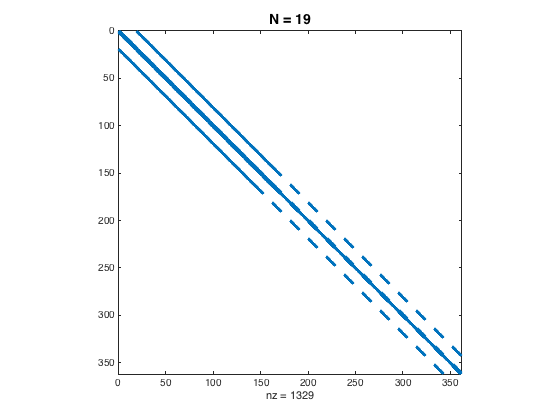
\includegraphics[scale=.5]{Figures/03_5_1.png}
            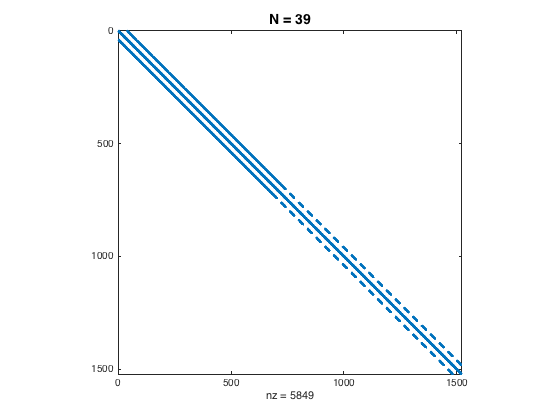
\includegraphics[scale=.5]{Figures/03_5_2.png}
        \end{center}

    \item % #6 Done
        Solve the PDE using your code with the right hand side
        \[
            f(x, y) = 1.
        \]

        The following code evalates the function from problem 4 for the
        given right hand side.
        The images produced are shown below.
        \lstinputlisting[language=Matlab, lastline=12]{H03_4.m}
        \begin{center}
            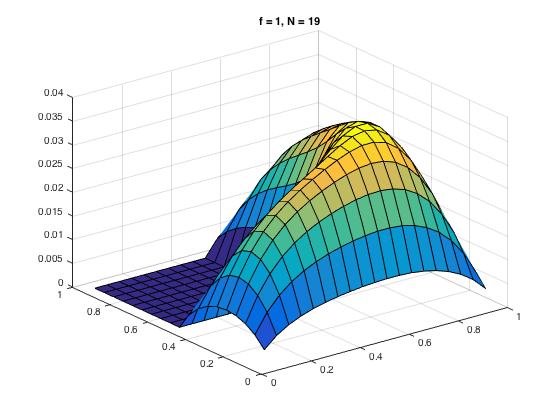
\includegraphics[scale=.5]{Figures/03_6_1.png}
            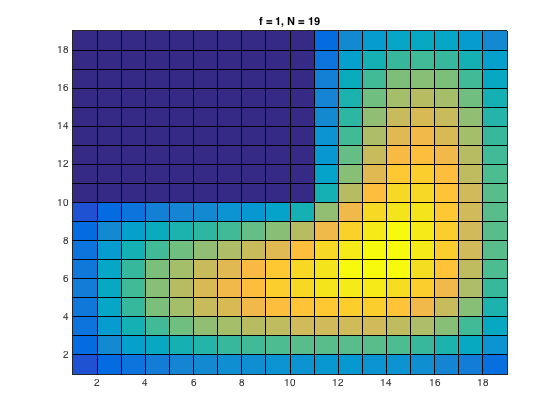
\includegraphics[scale=.5]{Figures/03_6_2.png}
            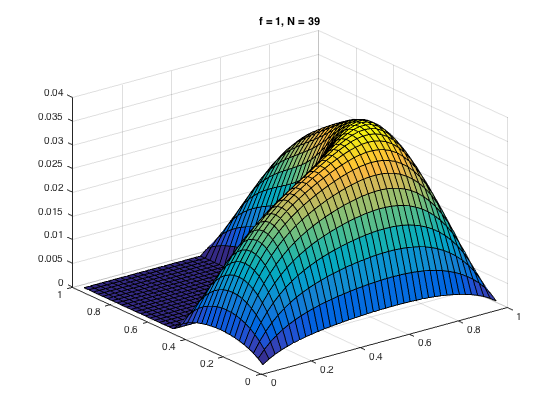
\includegraphics[scale=.5]{Figures/03_6_3.png}
            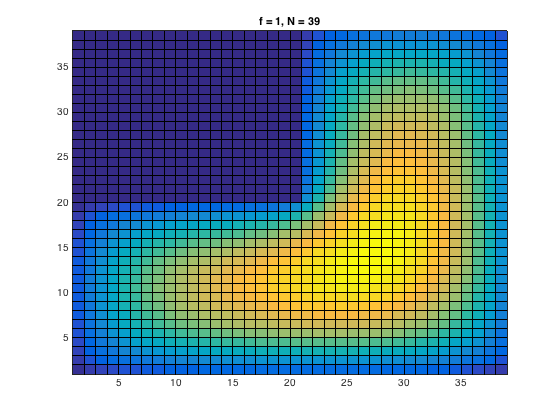
\includegraphics[scale=.5]{Figures/03_6_4.png}
        \end{center}

    \item % #7 Done
        Solve the PDE using your code with the right hand side
        \[
            f(x, y) = 2 exp\br{-(10x - 5)^2 - (10y - 5)^2}.
        \]

        The following code evalates the function from problem 4 for the
        given right hand side.
        The images produced are shown below.
        \lstinputlisting[language=Matlab, firstline=14, lastline=25]{H03_4.m}
        \begin{center}
            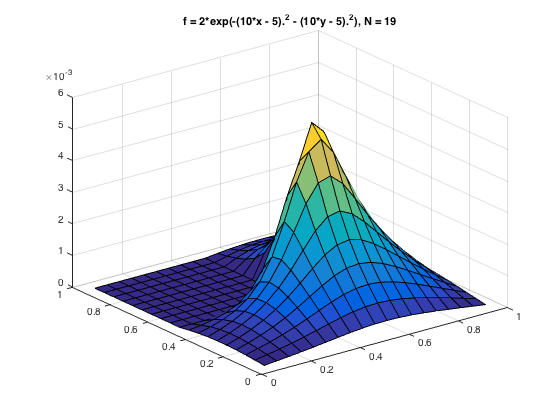
\includegraphics[scale=.5]{Figures/03_7_1.png}
            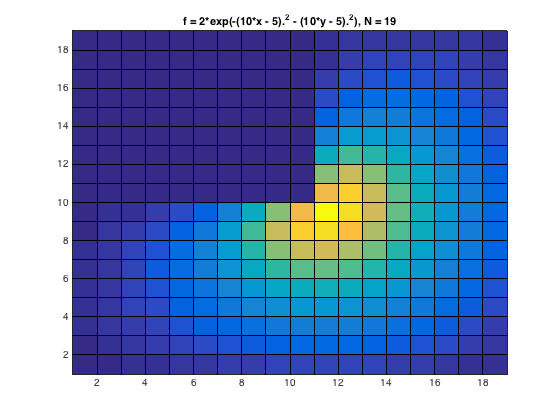
\includegraphics[scale=.5]{Figures/03_7_2.png}
            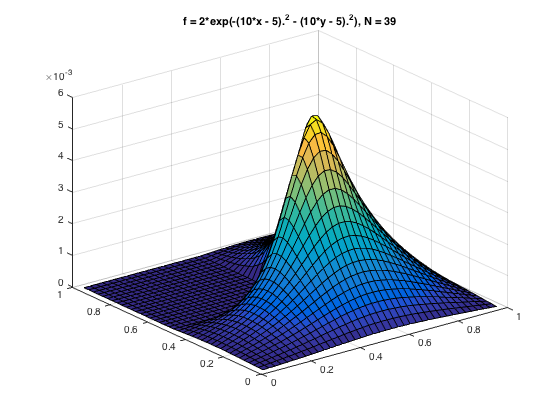
\includegraphics[scale=.5]{Figures/03_7_3.png}
            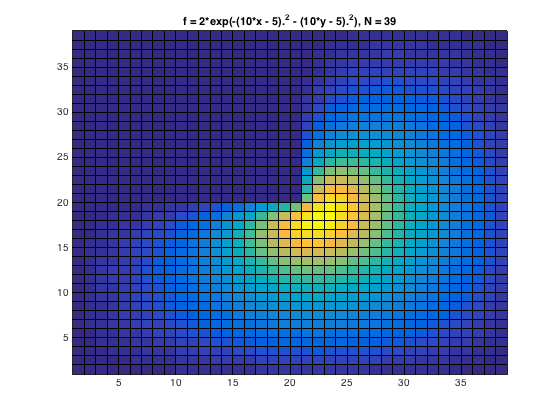
\includegraphics[scale=.5]{Figures/03_7_4.png}
        \end{center}

    \item % #8 Done
        Compute the Cholesky factorization of A is MATLAB: R = chol(A);
        where $R$ is an upper triangular matrix such that $A = R^T R$.
        For $N = 19$ and $N = 39$ produce a spy plot of $R$.
        Create a table showing the non-zeros in R for
        $N = 9, 19, 39, 79, 159, 319$.

        The following code is for problems 8 and 9.
        \lstinputlisting[language=Matlab, firstline=27]{H03_4.m}

        The following is the spy plots and table for problem 8.
        \begin{center}
            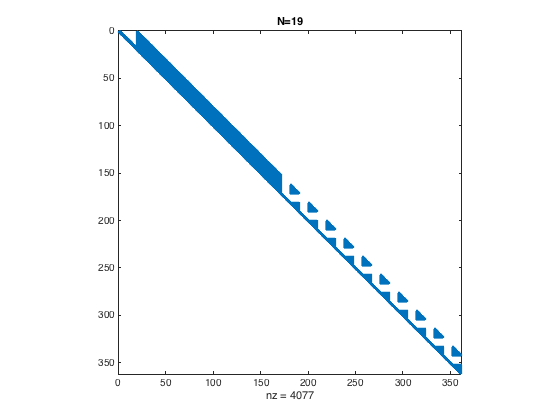
\includegraphics[scale=.5]{Figures/03_8_1.png}
            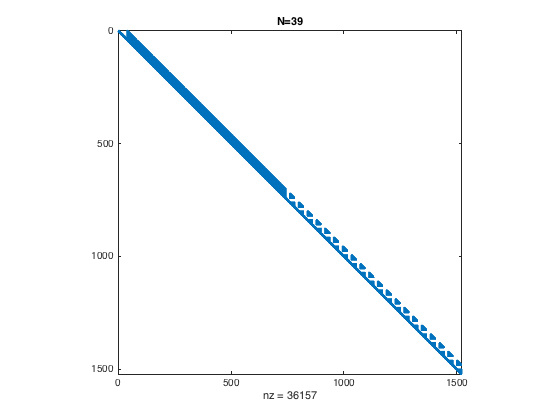
\includegraphics[scale=.5]{Figures/03_8_2.png}
        \end{center}

        \begin{verbatim}
            ans = 

                Var1     countsA  
                ____    __________

                9            412
                19           4077
                39          36157
                79     3.0432e+05
                159     2.4966e+06
                319     2.0225e+07
        \end{verbatim}

    \item % #9 Done
        Permute the matrix $A$ using the reverse Cuthill-Mckee algorithm in
        MATLAB: P = symrcm(A); B = A(P, P);
        Compute the Cholesky factorization of $B$ in MATLAB: R = chol(B);
        For $N = 19$ and $N = 39$ produce a spy plot of $R$.
        Create a table showing the non-zeros in R for
        $N = 9, 19, 39, 79, 159, 319$.

        The following is the spy plots and table for problem 9 generated by
        the code shown under problem 8.
        \begin{center}
            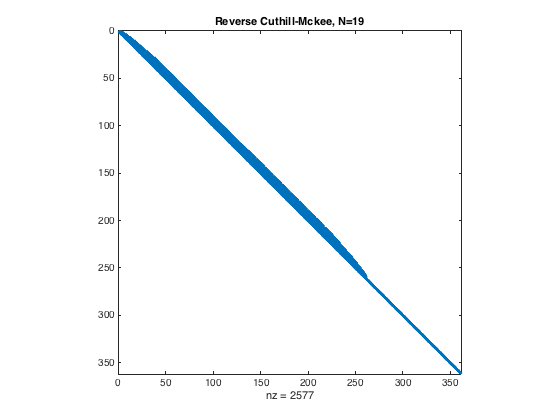
\includegraphics[scale=.5]{Figures/03_9_1.png}
            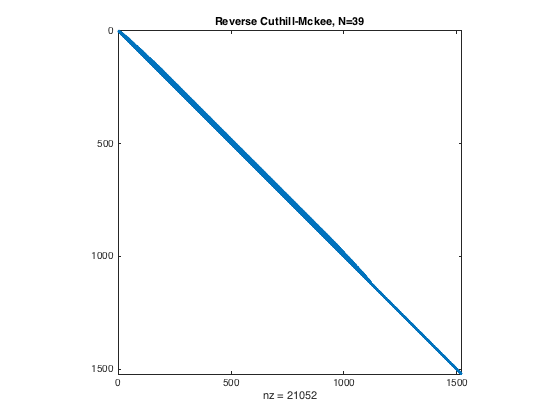
\includegraphics[scale=.5]{Figures/03_9_2.png}
        \end{center}
        \begin{verbatim}
            ans = 

                Var1     countsB  
                ____    __________

                9            302
                19           2577
                39          21052
                79      1.697e+05
                159     1.3618e+06
                319     1.0909e+07
        \end{verbatim}
\end{enumerate}
\end{document}
